\documentclass{article}
\usepackage[italian]{babel}

\usepackage{epigraph}
\usepackage{fontspec}
\usepackage{graphicx}
\usepackage[hidelinks]{hyperref}
\usepackage{verbatim}
\usepackage{graphicx}

\graphicspath{ {./images/} }

\title{
	\textbf{
		Birdazzone \\
	}
	\textbf{\large
		Relazione del progetto per l'insegnamento di \break
		Ingegneria del software
	}
}

\author{
	Paolo Ceroni (\#978232), \\
	Gabriele Crestanello (\#970352), \\
	Mattia Girolimetto (\#977478), \\
	Federica Grisendi (\#974711), \\
	Stefano Volpe (\#969766)
}

\date{
	Alma Mater Studiorum - Universit\`a di Bologna \\
	\today
}

\begin{document}

\maketitle

\epigraph{
	Engineering --- where the semi-skilled laborers execute the vision of those
	who think and dream. Hello, Oompa-Loompas of science.
}{\textit{Sheldon Cooper}}

\thispagestyle{empty}
\pagebreak

\tableofcontents

\pagebreak

\section{Descrizione del prodotto}

\subsection{\emph{Scope e backlog} di prodotto}

Le storie effettivamente svolte sono organizzate in epiche di origine.
All'interno di ciascuna epica, le storie sono organizzate in ordine decrescente
di priorità.

\subsubsection{Preparazione tecnica}

\begin{itemize}
	\item \#0 Partita a Scrumble
	\item \#1 Ambiente di sviluppo CAS
	\item \#2 Configurazione dipendente dalle tecnologie
	\item \#3 Ambiente di \emph{test}
\end{itemize}

\subsubsection{Indovinare la ``ghigliottina''}

\begin{itemize}
	\item \#4 ``Come giocatore da casa, voglio visualizzare al classifica di chi ha
	      indovinato per vedere la posizione mia e dei miei amici''
	\item \#5 ``Come giocatore da casa, voglio essere a conoscenza della soluzione
	      della partita per capire se ho indovintato o meno''
	\item \#6 ``Come giocatore da casa, voglio che solo i giocatori che hanno davvero
	      indovinato vengano mostrati in classifica''
	\item \#7 ``Come appassionato curioso, voglio visualizzare dove si trovano i
	      giocatori che hanno indovinato per studiare la loro demografia''
	\item \#8 ``Come appassionato curioso, voglio filtrare i risultati temporalmente
	      per studiare uno specifico intervallo di tempo''
	\item \#9 ``Come appassionato curioso, voglio vedere lo storico dei risultati
	      complessivi delle partite per studiare la loro evoluzione''
\end{itemize}

\subsubsection{Indovinare la ``reazione a catena''}

Questa epica, in seguito abbandonata dal cliente, ha dato origine a un gioco
segnaposto: Birdazzone, in cui si indovina in quale città una certa foto su
Twitter è stata scattata. Le storie di questa epica sono le stesse della
Ghigliottina.

\subsubsection{Fantacitorio}

\begin{itemize}
	\item \#10 ``Come giocatore del Fantacitorio, voglio vedere quanti punti ciascun
	      politico ha realizzato per capire come stia andando la partita''
	\item \#11 ``Come giocatore del Fantacitorio, voglio vedere le squadre degli altri
	      giocatori per poterle confrontare con la mia''
	\item \#12 ``Come giocatore del Fantacitorio, voglio vedere statistiche aggiuntive
	      sui politici per strategizzare meglio''
\end{itemize}

\subsubsection{Scacchi contro la folla}

\begin{itemize}
	\item \#13 ``Come giocatore di scacchi, voglio poter sfidare una folla di
	      utenti Tweeter per giocare una partita le cui mosse avversarie siano
	      decise a maggioranza''
	\item \#14 ``Come giocatore di scacchi, voglio poter condividere le mie mosse
	      su Twitter per rendere le mie partite pubbliche''
\end{itemize}

\subsection{Diagramma dei casi d'uso}

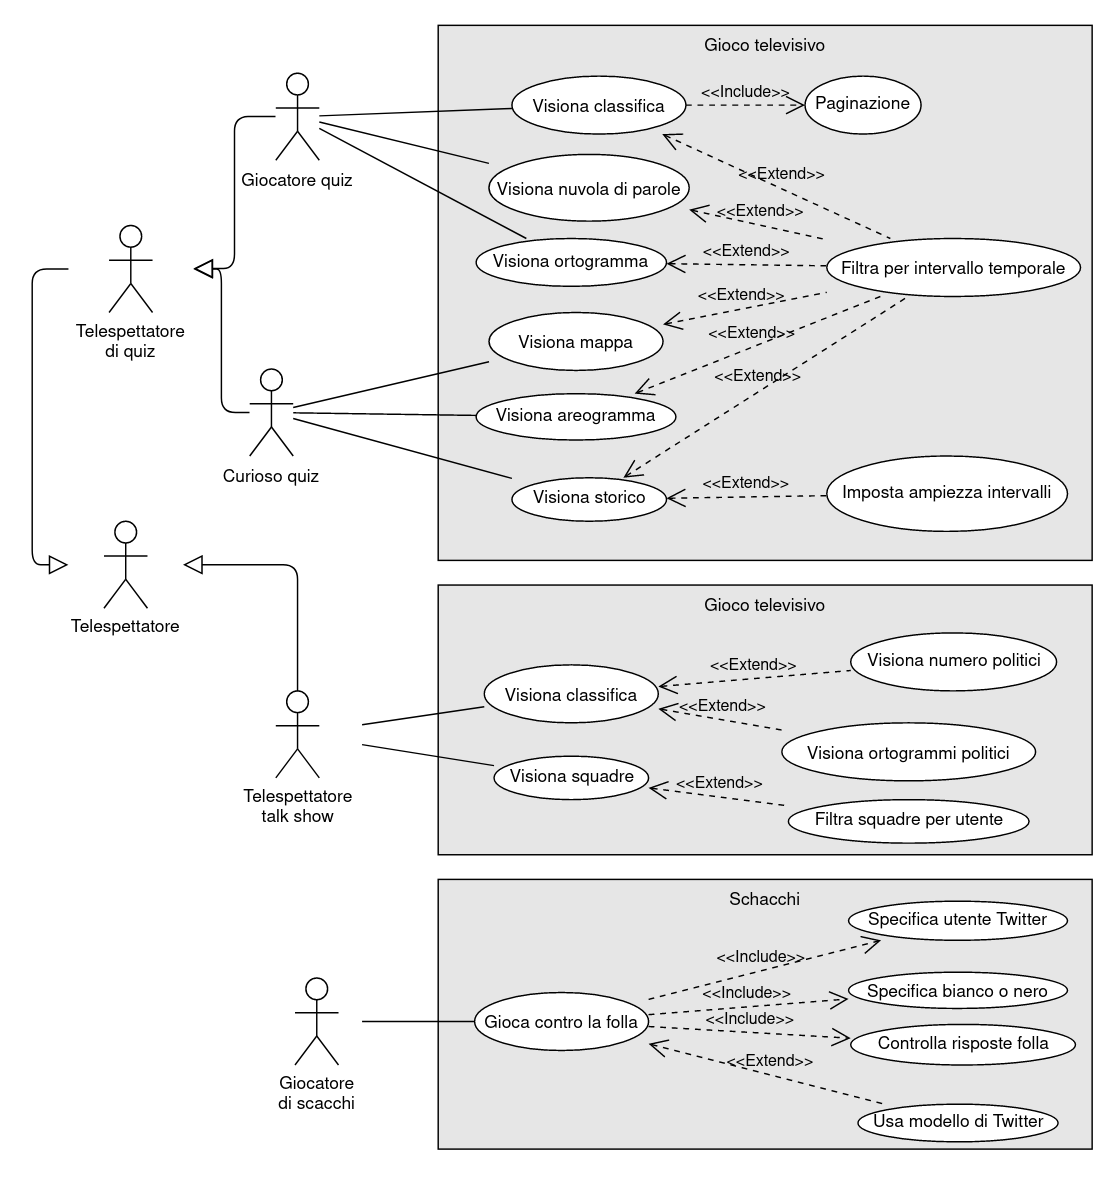
\includegraphics[width=\textwidth]{use-cases}

\subsection{Diagramma delle classi o degli oggetti}

Golang supporta la programmazione orientata agli oggetti, ma non le classi.
TypeScript supporta le classi, ma come ragionevole convenzione di progetto è
stata fatta la scelta di evitare la programmazione a oggetti durante lo
sviluppo front-end, che descrive solo una interfaccia grafica, e non la logica
di business. Ecco un diagramma pseudo-UML che descrive invece il progetto
back-end:

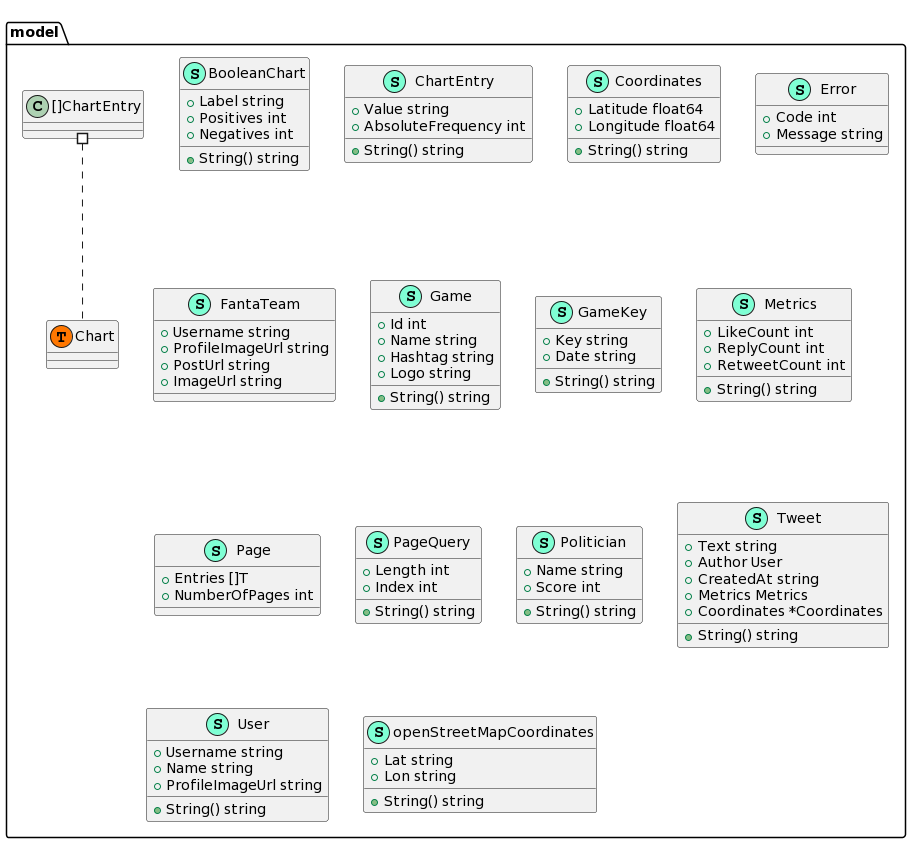
\includegraphics[width=\textwidth]{backend-model}
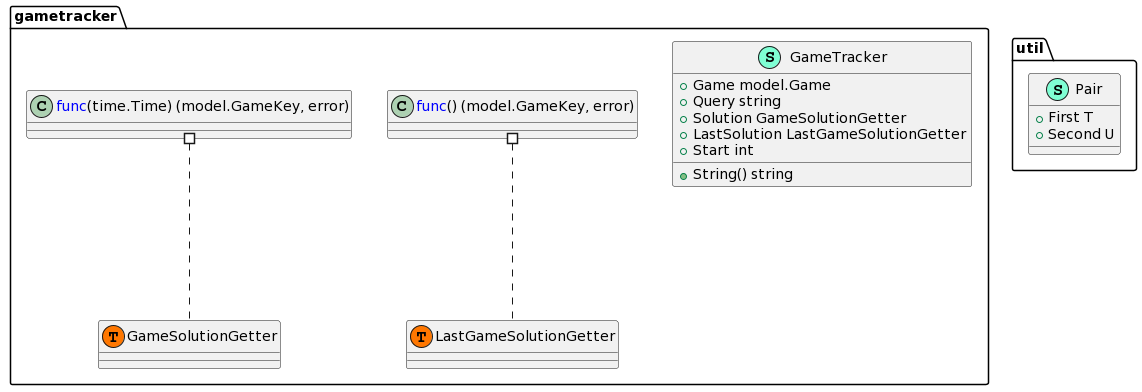
\includegraphics[width=\textwidth]{backend-gametracker-util}
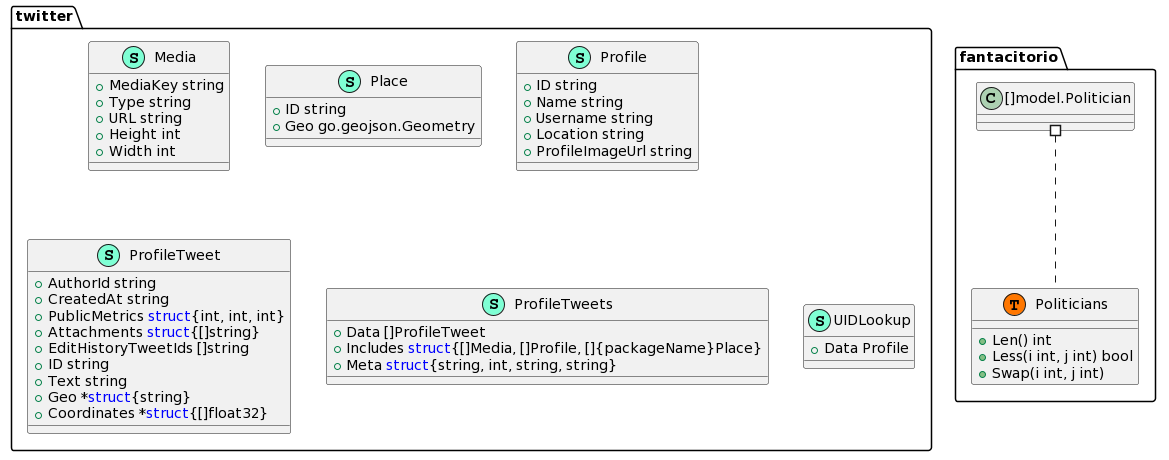
\includegraphics[width=\textwidth]{backend-twitter-fantacitorio}

\section{\emph{Sprint} 0}

\subsection{\emph{Sprint goal}}

Lo sprint goal per lo sprint 0 è la "preparazione" dell'intero progetto.

\subsection{\emph{Sprint backlog}}

Lo sprint backlog è consistito di due storie, entrambe tecniche: \#0 e \#1.

\subsection{\emph{Definition of done}}

La definition of done del progetto è stata definita proprio in questo sprint.
Non è stata usata per verificare la qualità del lavoro svolto poiché sono state
effettuate solo prove tecniche. Si ha comunque fatto uso di una definition of
done "giocattolo" per la partita di prova a Scrumble.

\subsection{\emph{Test} di ciascuna storia}

Essendoci state solo storie teniche, il sistema di test non era ancora
disponibile nello sprint 0.

\subsection{\emph{Burndown} dello sprint}

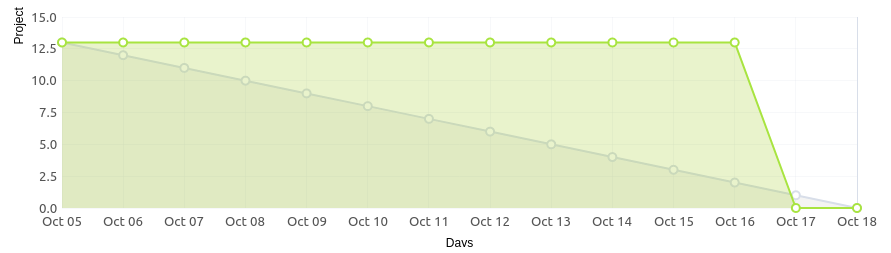
\includegraphics[width=\textwidth]{burndown-0}

\subsection{Retrospettiva con \emph{Essence}}

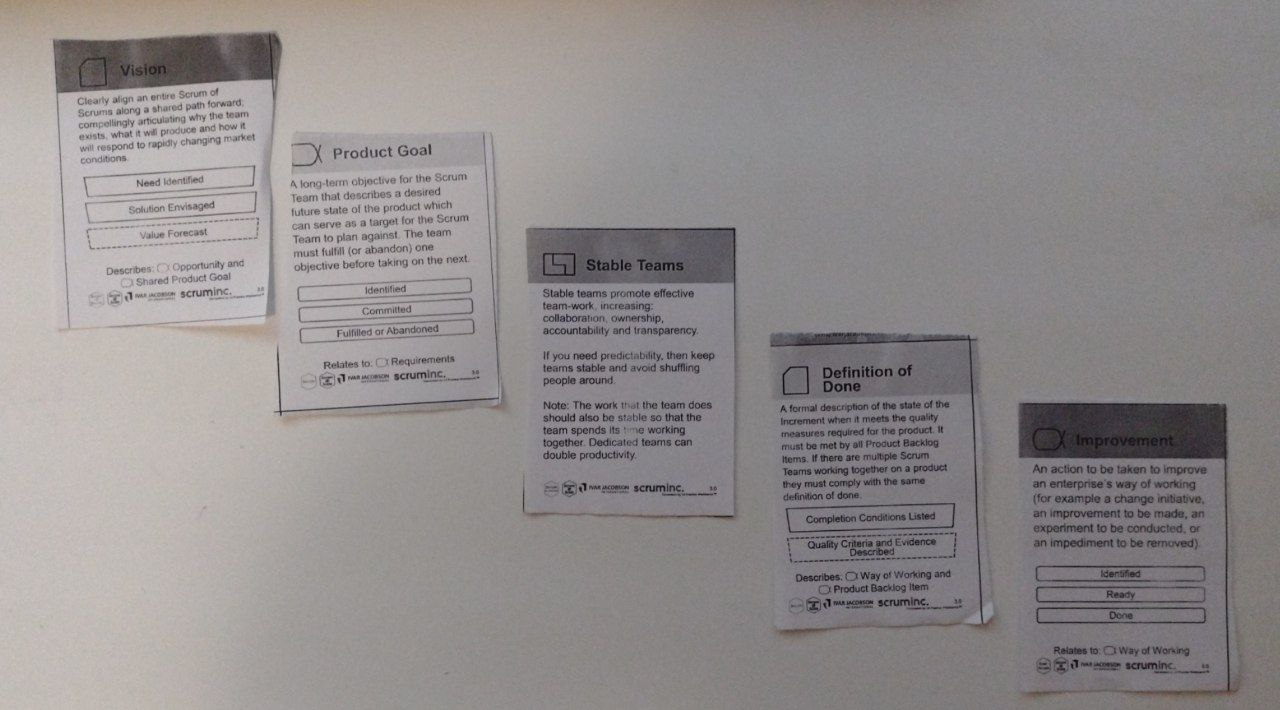
\includegraphics[width=\textwidth]{essence-0}

\section{\emph{Sprint} 1}

\subsection{\emph{Sprint goal}}

Il tema di questo sprint è "Last Word Guessing Games (A)".

\subsection{\emph{Sprint backlog}}

Lo sprint backlog è composto dalle storie \#2, \#3, \#4.

\subsection{\emph{Definition of done}}

La definition of done definita durante lo sprint 0 è stata rispettata per tutte
le storie dello sprint 1.

\subsection{\emph{Test} di ciascuna storia}

\#2 e \#3 sono storie tecniche. Per \#4, abbiamo testato l'analisi del testo dei
Tweet in \verb!tvgames/tvgames_test.go!.

\subsection{\emph{Burndown} dello sprint}

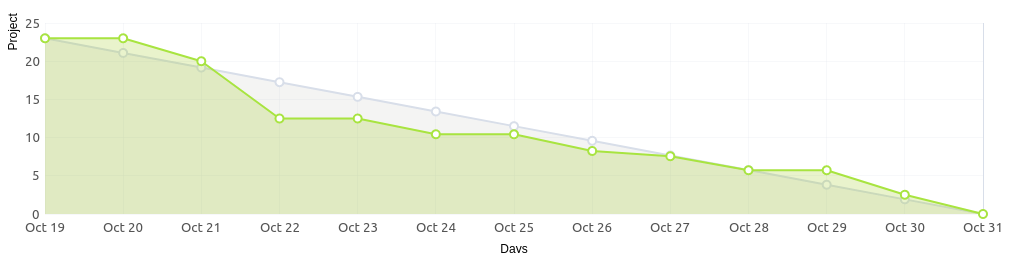
\includegraphics[width=\textwidth]{burndown-1}

\subsection{Retrospettiva con \emph{Essence}}

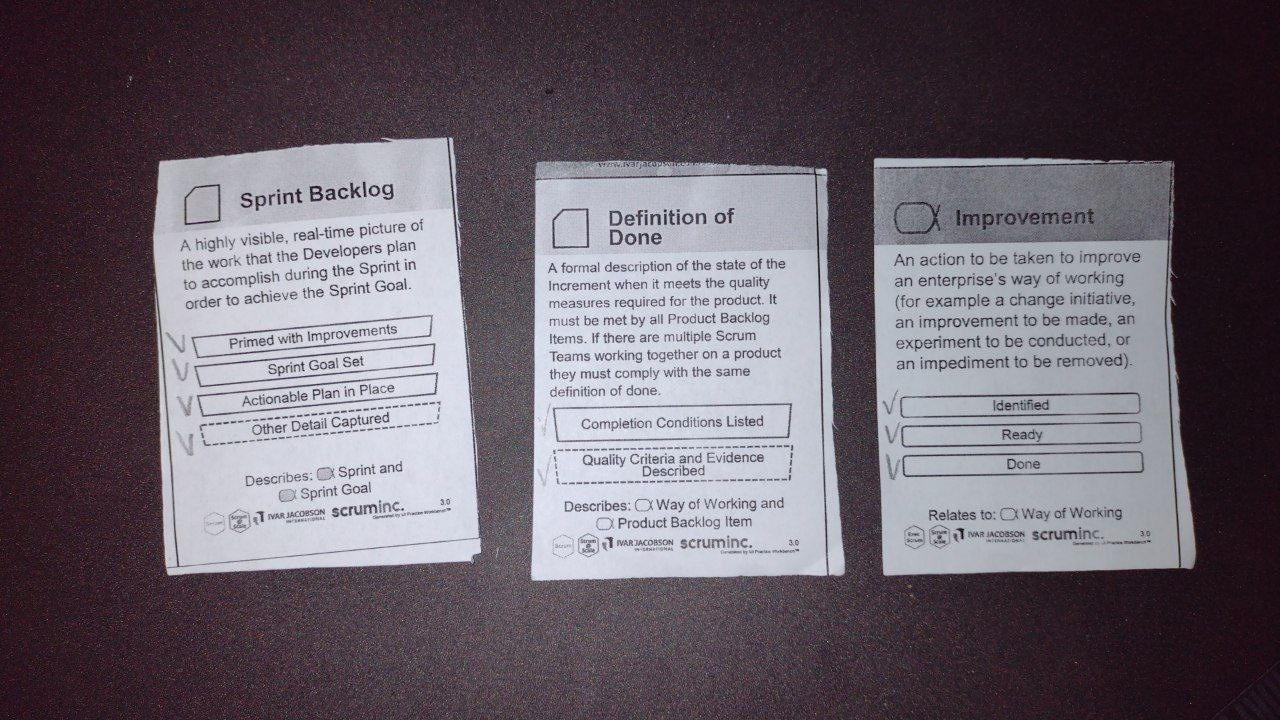
\includegraphics[width=\textwidth]{essence-1}

\section{\emph{Sprint} 2}

\subsection{\emph{Sprint goal}}

Il tema di questo sprint è "Last Word Guessing Games (B)".

\subsection{\emph{Sprint backlog}}

Le storie coinvolte sono state \#5 e \#6.

\subsection{\emph{Definition of done}}

Le storie \#5 e \#6. Non hanno tutte superato la definition of
done: il frontend non gestiva tutti i casi particolari del backend, né tutti i
vincoli temporali. Il backend superava i propri test solo in alcune fasce
orarie. Questo ha causato del debito tecnico, che però è stato recuperato dopo
la recensione e prima della fine dello sprint.

\subsection{\emph{Test} di ciascuna storia}

Queste cinque storie sono testate in \verb!tvgames/tvgames_test.go! e
\verb!model/model_test.go!.

\subsection{\emph{Burndown} dello sprint}

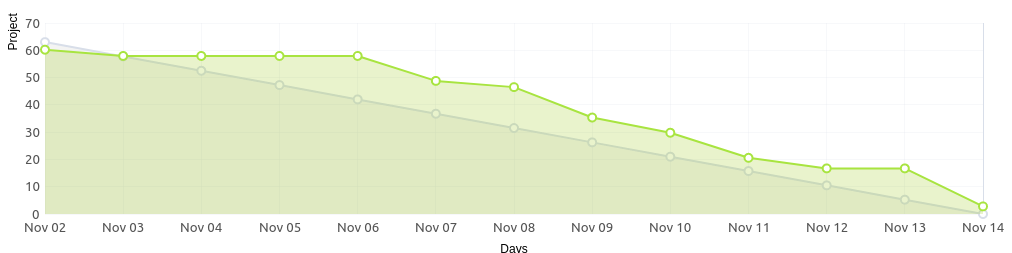
\includegraphics[width=\textwidth]{burndown-2}

\subsection{Retrospettiva con \emph{Essence}}

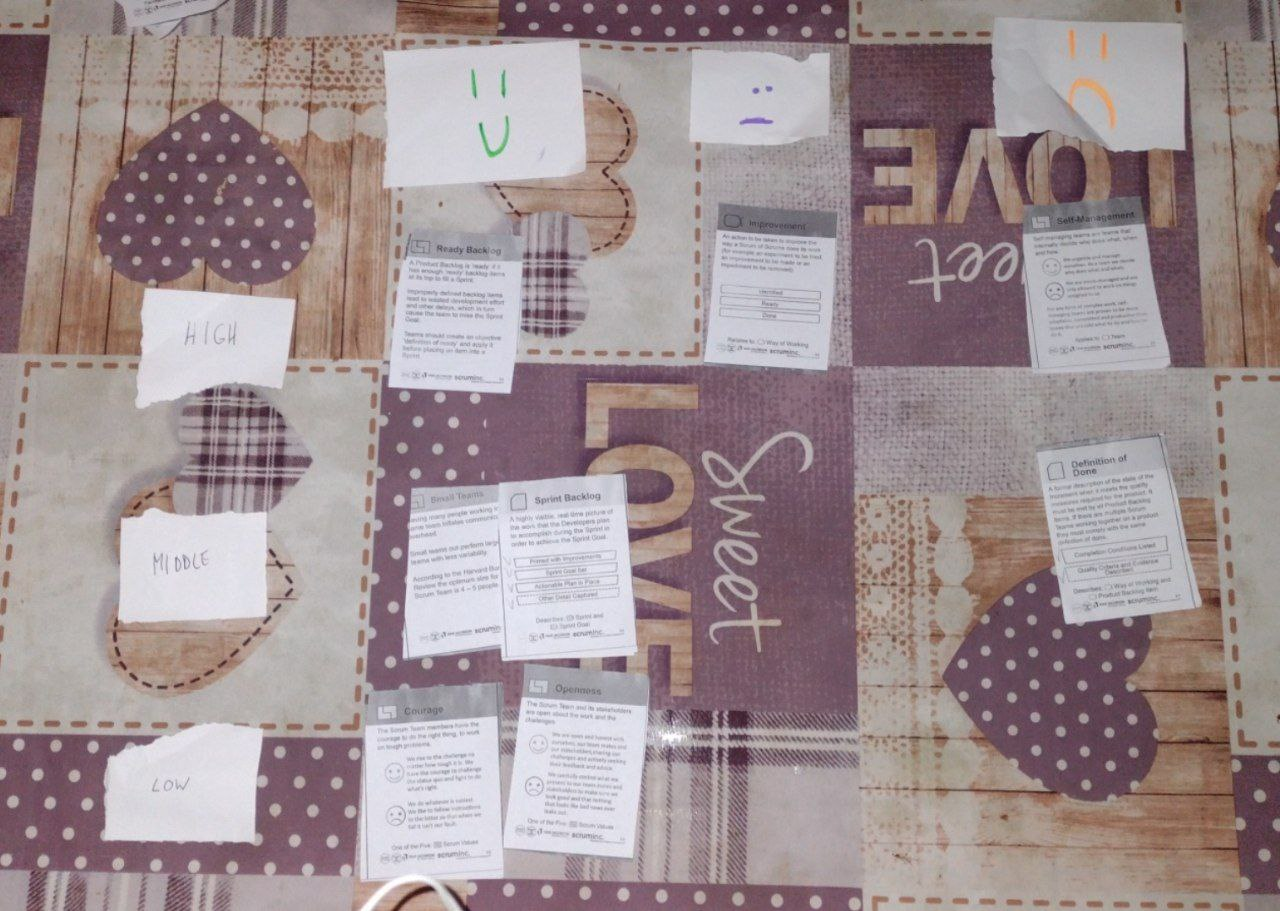
\includegraphics[width=\textwidth]{essence-2}

\section{\emph{Sprint} 3}

\subsection{\emph{Sprint goal}}

Lo sprint goal si intitolava "A Time and a Place for Everythin". Lo sprint
infatti verteva sui luoghi (la mappa) e sui filtri temporali.

\subsection{\emph{Sprint backlog}}

Le storie coinvolte sono state \#7, \8 e \#9.

\subsection{\emph{Definition of done}}

In questo sprint la definition of done è stata rispettata. Perché i test
passavano tutti. Solo in seguito ci siamo accorti di tutti i casi particolari
non gestiti.

\subsection{\emph{Test} di ciascuna storia}

Queste cinque storie sono testate in \verb!tvgames/tvgames_test.go! e
\verb!model/model_test.go!.

\subsection{\emph{Burndown} dello sprint}

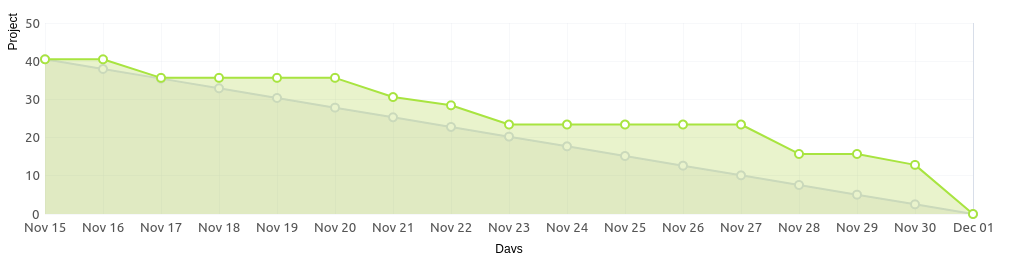
\includegraphics[width=\textwidth]{burndown-3}

\subsection{Retrospettiva con \emph{Essence}}

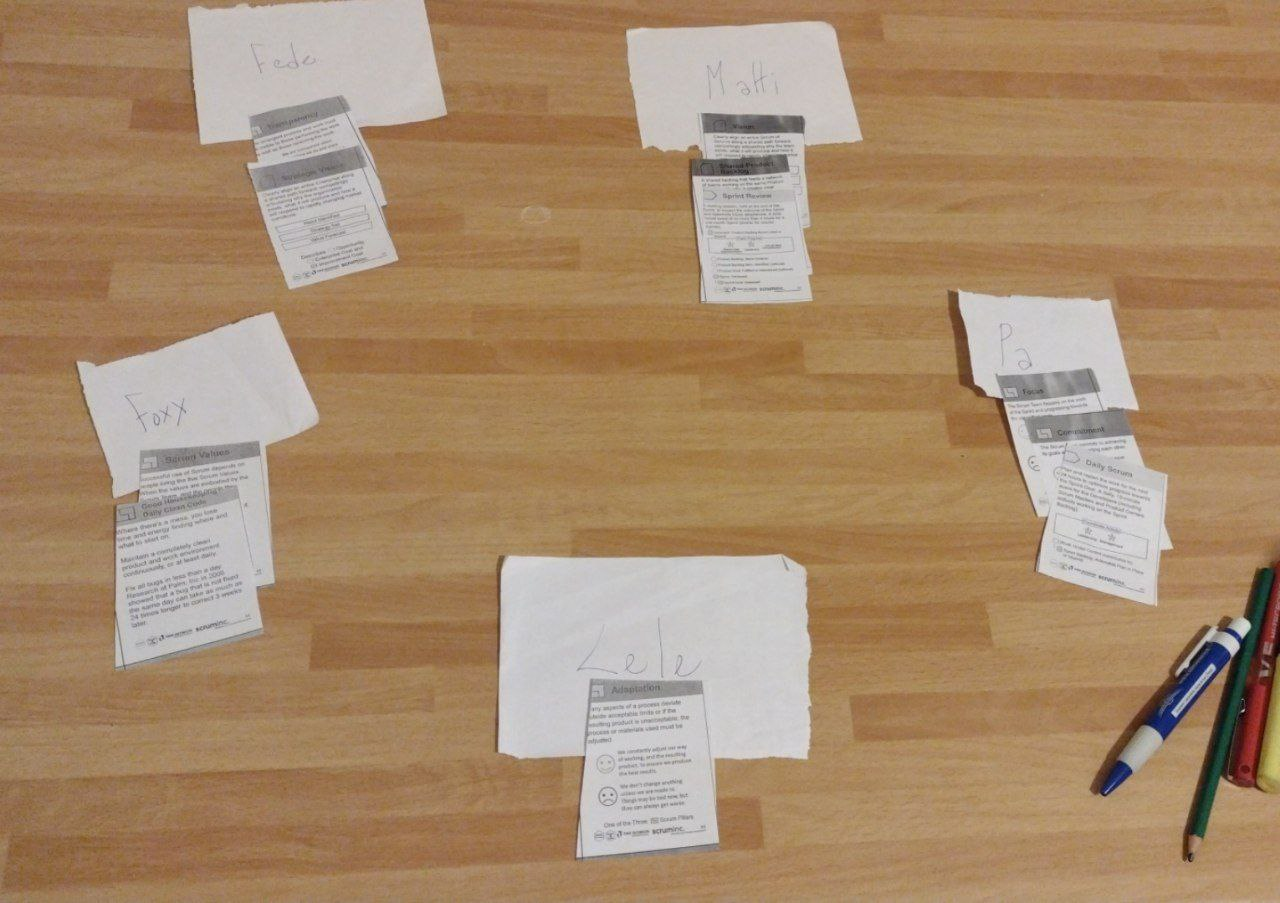
\includegraphics[width=\textwidth]{essence-3}

\section{\emph{Sprint} 4}

\subsection{\emph{Sprint goal}}

\subsection{\emph{Sprint backlog}}

\subsection{\emph{Definition of done}}

\subsection{\emph{Test} di ciascuna storia}

\subsection{\emph{Burndown} dello sprint}

\subsection{Retrospettiva con \emph{Essence}}

\section{Qualità del codice}

\section{Processo seguito}

\subsection{Numero e durata degli sprint}

\subsection{Autodescrizione del \emph{team}}

\subsection{Risultato dello Scrumble iniziale}

\subsection{Sintesi dei dati di \emph{Gitinspector}}

\subsection{Retrospettiva finale con \emph{Essence}}

\subsection{Diagramma del \emph{deployment} del prodotto}

\section{Demo}

\section{Artefatti}

\end{document}
